\documentclass[aspectratio=169, xcolor=dvipsnames]{beamer}


\usepackage[utf8]{inputenc}
\usepackage{amsmath}
\usepackage{amsfonts}
\usepackage{amssymb}
\usepackage{graphicx}
\usepackage{ragged2e}  % `\justifying` text
\usepackage{booktabs}  % Tables
\usepackage{tabularx}
\usepackage{tikz}      % Diagrams
\usetikzlibrary{positioning}
\usetikzlibrary{calc, shapes, backgrounds}
\usepackage{amsmath}
\usepackage{amssymb}
\usepackage{dsfont}
\usepackage{url}       % `\url
\usepackage{listings}  % Code listings
\usepackage[T1]{fontenc}
\usepackage{xcolor}
\usepackage{colortbl}
\usepackage{multimedia}

\usepackage{theme/beamerthemehbrs}

\newcolumntype{C}{>{\centering\arraybackslash}m}
\newcolumntype{g}{>{\columncolor{gray}}c}

\author[H. Walli]{Hasnainali Walli}
\title{Lifelong Action Learning for Socially Assistive Robots}
%\subtitle{Subtitle of presentation}
\institute[HBRS]{Hochschule Bonn-Rhein-Sieg}
\date{November 28th, 2022}
\subject{Master's Thesis Defense}

% leave the value of this argument empty if the advisors
% should not be included on the title slide
\def\advisors{Prof. Dr. Paul G. Plöger, Prof. Dr. Sebastian Houben, Alex Mitrevski}

% \thirdpartylogo{path/to/your/image}


\begin{document}
{
\begin{frame}
\titlepage
\end{frame}
}


\section{Introduction}
%\subsection{A subsection}

\begin{frame}{Motivation}
      \framesubtitle{}%
      
      \begin{itemize}
              \item Action recognition is a key function for socially assistive robots
              \item \textbf{Challenge}: Conventional models' inability to learn new actions
              \item How can robotic systems learn new actions without forgetting?
      \end{itemize}
      \vfill
      {\footnotesize
      \centering
      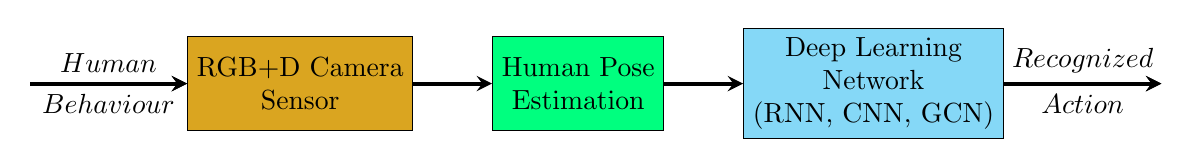
\begin{tikzpicture}
              \node[draw, align=center, fill=Goldenrod, minimum width=1cm, minimum height=1.2cm]  (cam) at (0,0) {RGB+D Camera\\ Sensor};
              \node[draw, align=center, fill=SpringGreen, minimum width=1cm, minimum height=1.2cm, right= 1cm of cam]  (pos) {Human Pose\\ Estimation};
              \node[draw, align=center, fill=ProcessBlue!50, minimum width=1cm, minimum height=1.2cm, right= 1cm of pos]  (nn) {Deep Learning\\ Network\\(RNN, CNN, GCN)};
              
              \draw[stealth-,  line width=0.05cm] (cam.west) -- ++ (-2,0) node[midway,above]{$Human$};
              \draw[stealth-,  line width=0.05cm] (cam.west) -- ++ (-2,0) node[midway,below]{$Behaviour$};
              
              \draw[-stealth,  line width=0.05cm] (cam.east) -- (pos.west);
              \draw[-stealth,  line width=0.05cm] (pos.east) -- (nn.west);
              
              \draw[-stealth,  line width=0.05cm] (nn.east) -- ++ (2,0) node[midway,above]{$Recognized$};
              \draw[-stealth,  line width=0.05cm] (nn.east) -- ++ (2,0) node[midway,below]{$Action$};
      \end{tikzpicture}
      }
\end{frame}

\begin{frame}{Lifelong Action Learning}
      \framesubtitle{}%
      
      \begin{itemize}
              \item Robotic systems fine-tune their knowledge with experience
              \item New actions are learnt while retaining the knowledge of the previous actions
              \item Concept of lifelong action learning was explored in the context of CRI
              \item \textbf{Objectives}:
              \begin{itemize}
                  \item \small Develop an action learning model using incremental learning
                  \item \small Integrate model on QTRobot for the MigrAVE project
              \end{itemize}
      \end{itemize}
\end{frame}

\begin{frame}{Lifelong Action Learning}
      \framesubtitle{}%
      \begin{figure}[h!]
      \centering
      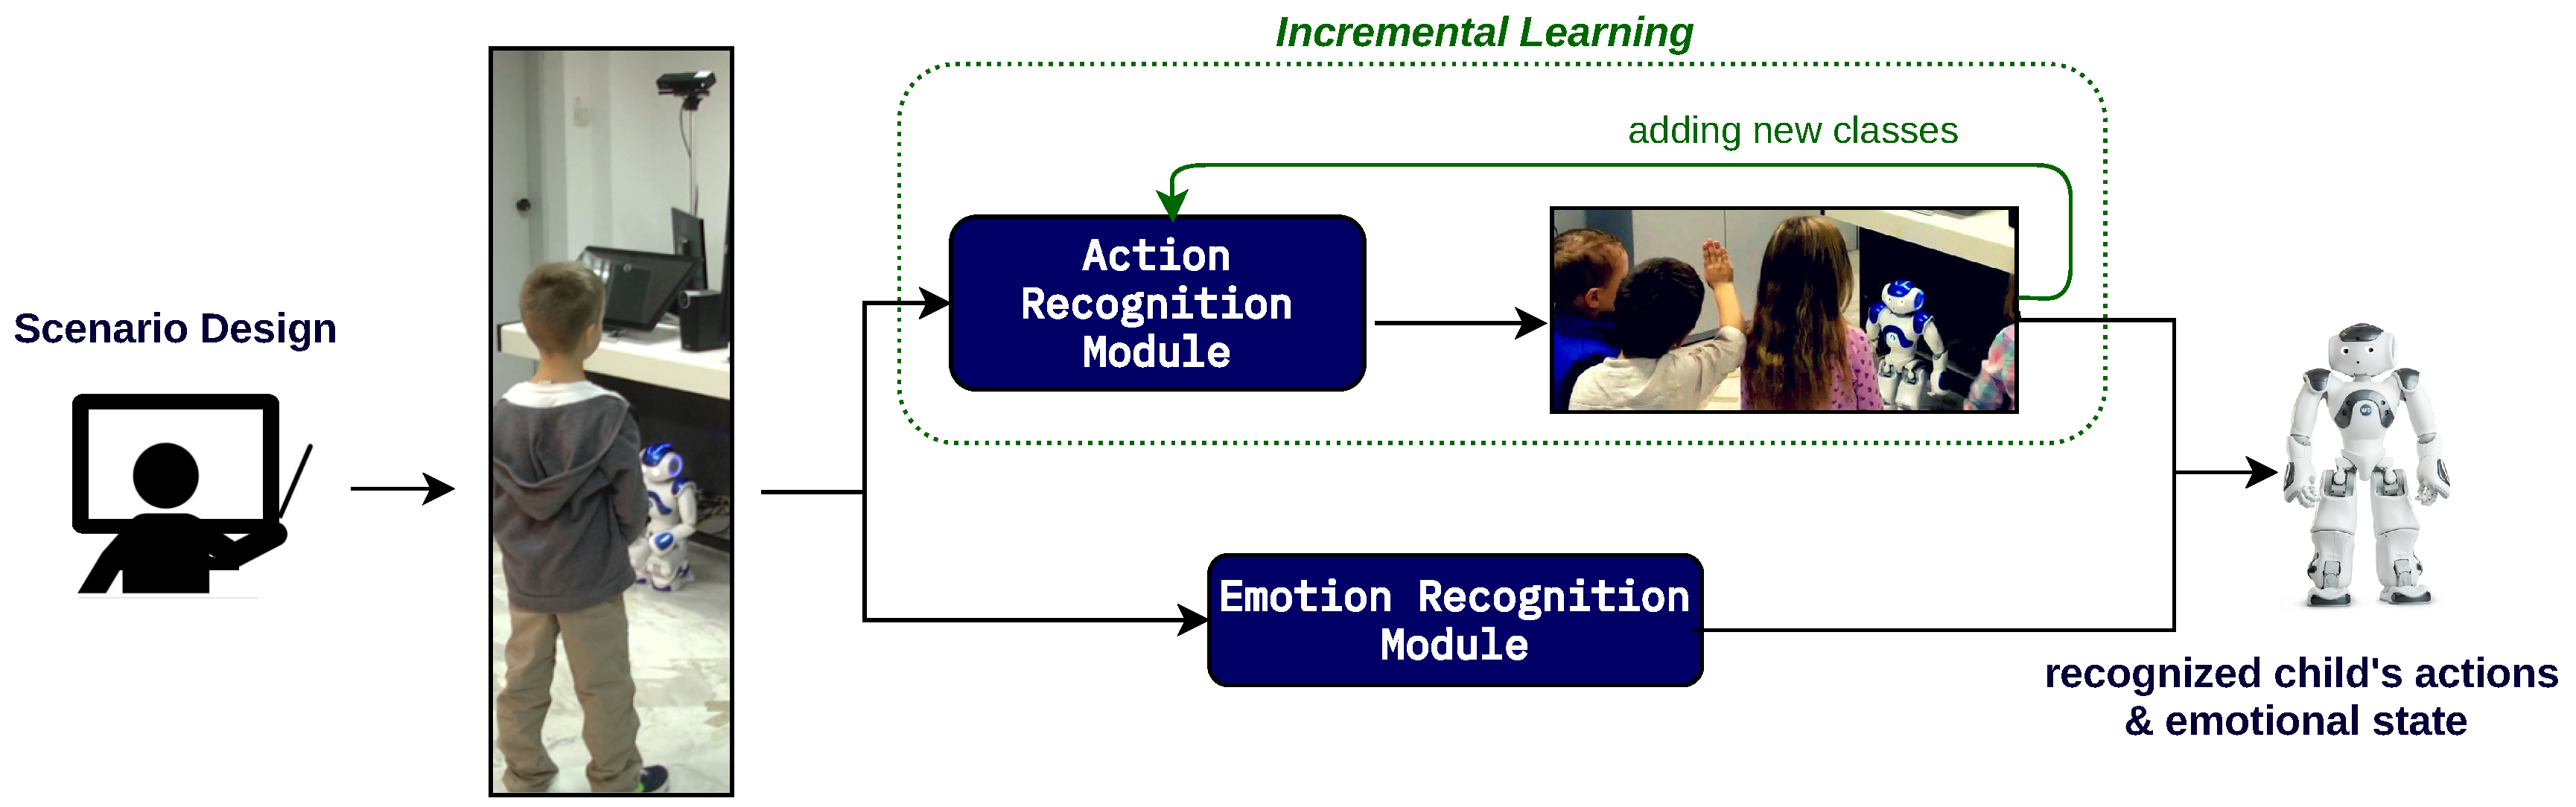
\includegraphics[width=0.9\textwidth]{images/IL_pipeline.png} 
      \caption{Incremental learning pipeline for action and emotion recognition\footnotemark}
      \end{figure} 
      \footnotetext{N. Efthymiou, P. P. Filntisis, G. Potamianos, and P. Maragos, “Visual Robotic Perception System with Incremental Learning for Child–Robot Interaction Scenarios,” Technologies, vol. 9, no. 86, November 2021.}
\end{frame}

\begin{frame}{Lifelong Action Learning}
      \framesubtitle{}%
      
      \begin{figure}[h!]
      \centering
      \begin{tikzpicture}
              \draw[red,thick,dashed] (0,0) ellipse (3cm and 1cm);
              \node(a){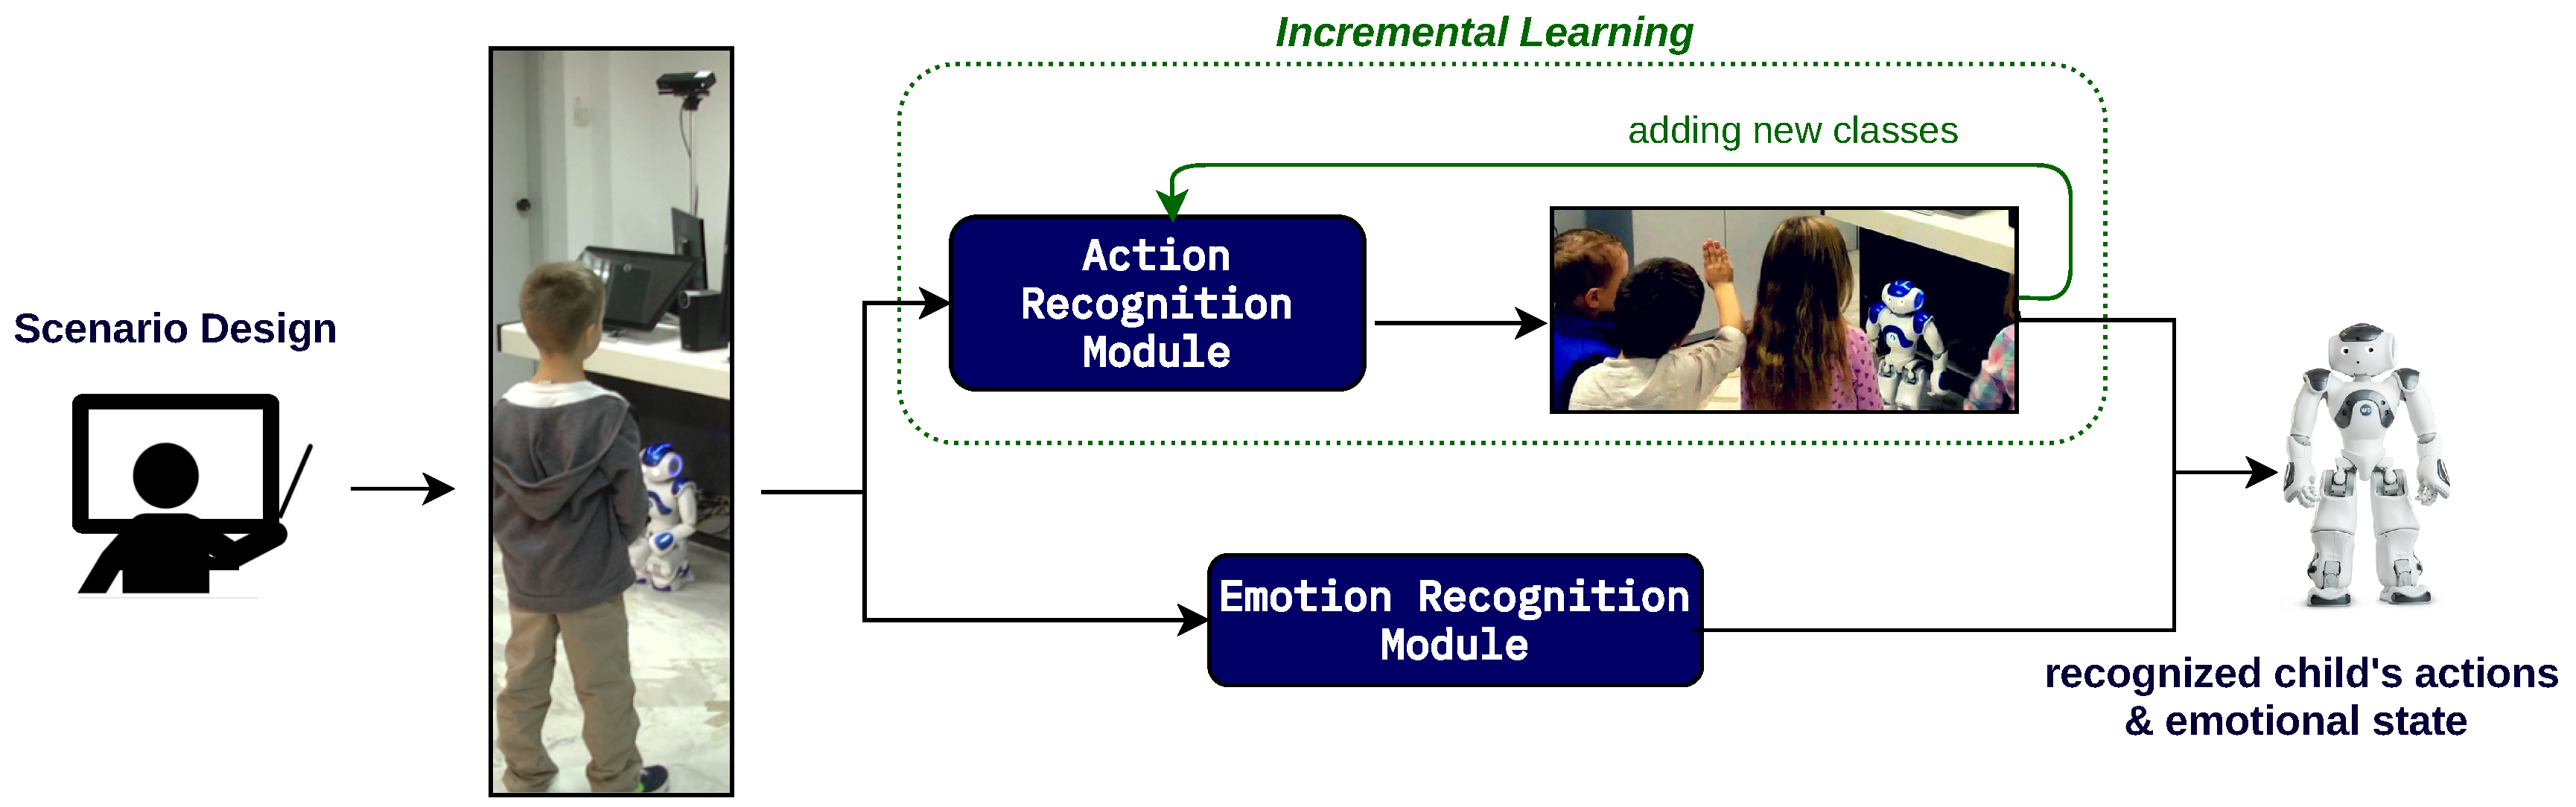
\includegraphics[width=0.9\textwidth]{images/IL_pipeline.png}};
              \node at (a.center) [draw, red, line width=3pt, ellipse, minimum width=200pt, minimum height=80pt, xshift=30pt, yshift=21pt]{};
      \end{tikzpicture}
      \caption{Incremental learning pipeline for action and emotion recognition\footnotemark}
      \end{figure} 
      \footnotetext{N. Efthymiou, P. P. Filntisis, G. Potamianos, and P. Maragos, “Visual Robotic Perception System with Incremental Learning for Child–Robot Interaction Scenarios,” Technologies, vol. 9, no. 86, November 2021.}
\end{frame}

\begin{frame}{Lifelong Action Learning}
      \framesubtitle{}%
      
      \begin{columns}
      \column{.5\textwidth}
      \begin{block}{Their Approach}
              \begin{itemize}
                  \item RGB+D and Optical Flow data
                  \item TSN Network
                  \item iCaRL Algorithm
                  \item BabyRobot Dataset
              \end{itemize}
      \end{block}
      
      \column{0.5\textwidth}
      \begin{block}{Our Approach}
              \begin{itemize}
                  \item 3D Skeleton data
                  \item CTR-GCN Network
                  \item BiC Algorithm
                  \item NTU RGB+D Dataset
              \end{itemize}
      \end{block}
      \end{columns}
\end{frame}

\begin{frame}{Our Approach}
      \framesubtitle{Methodology}%
      
      \begin{columns}
      \column{0.5\textwidth}
      \vspace{-0.75cm}
      \begin{enumerate}
              \item Perform comparative analysis on skeleton-based action recognition networks
              \item Perform comparative analysis on class-incremental learning algorithms
              \item Integrate final model on QTRobot
      \end{enumerate}
      
      \column{0.5\textwidth}
      \begin{figure}[ht!]
            \centering
            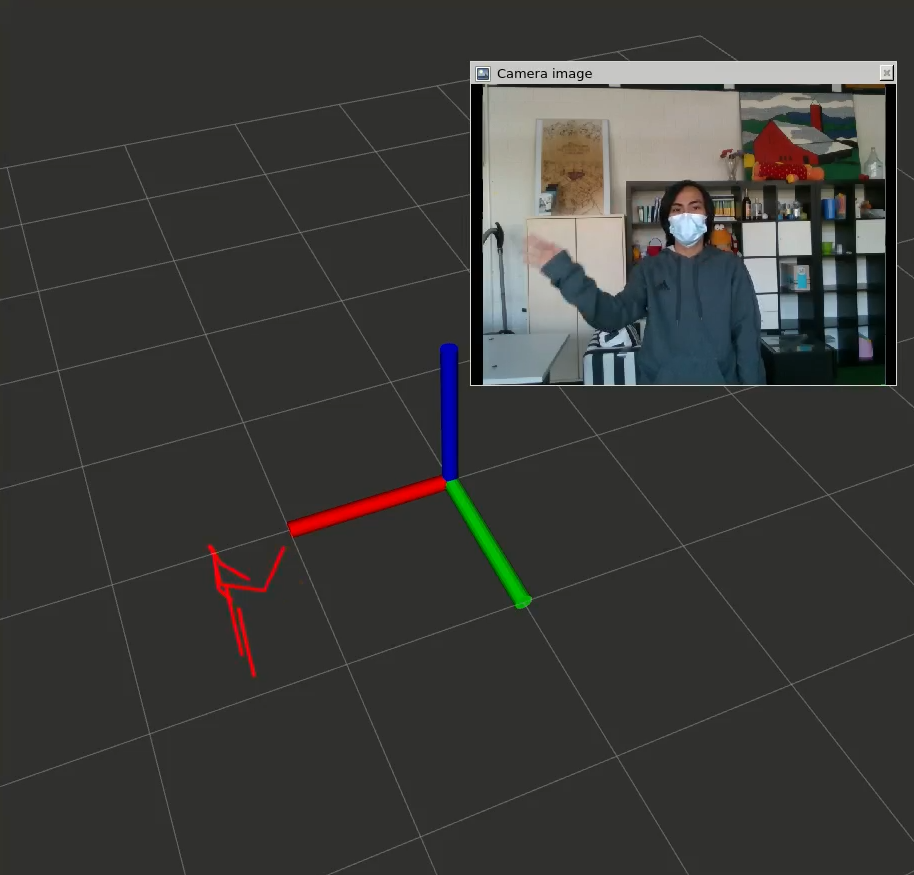
\includegraphics[width=0.7\textwidth]{images/waving_action_recognition.png}
            \caption{Hand waving action visualized in RVIZ}
      \end{figure}   
      \end{columns}
\end{frame}

\section{Comparative Analysis: Action Recognition}

\begin{frame}{NTU Dataset}
      \framesubtitle{}%
      
      \vspace{-0.75cm}
      \begin{columns}
      \column{.45\textwidth}
      \begin{itemize}
            \item Features 120 everyday actions
            \item 40 subjects; 3 cameras; 2 demos
            \item 25 skeletal joints tracked
            \item Evaluation:
            \begin{itemize}
                  \item Cross-Subject Accuracy: train on 20 subjects; test on 20 subjects
                  \item Cross-View Accuracy: train using 2 views; test on 1 view
            \end{itemize}
      \end{itemize}
      
      \column{.55\textwidth}
      \begin{figure}[ht!]
            \centering
            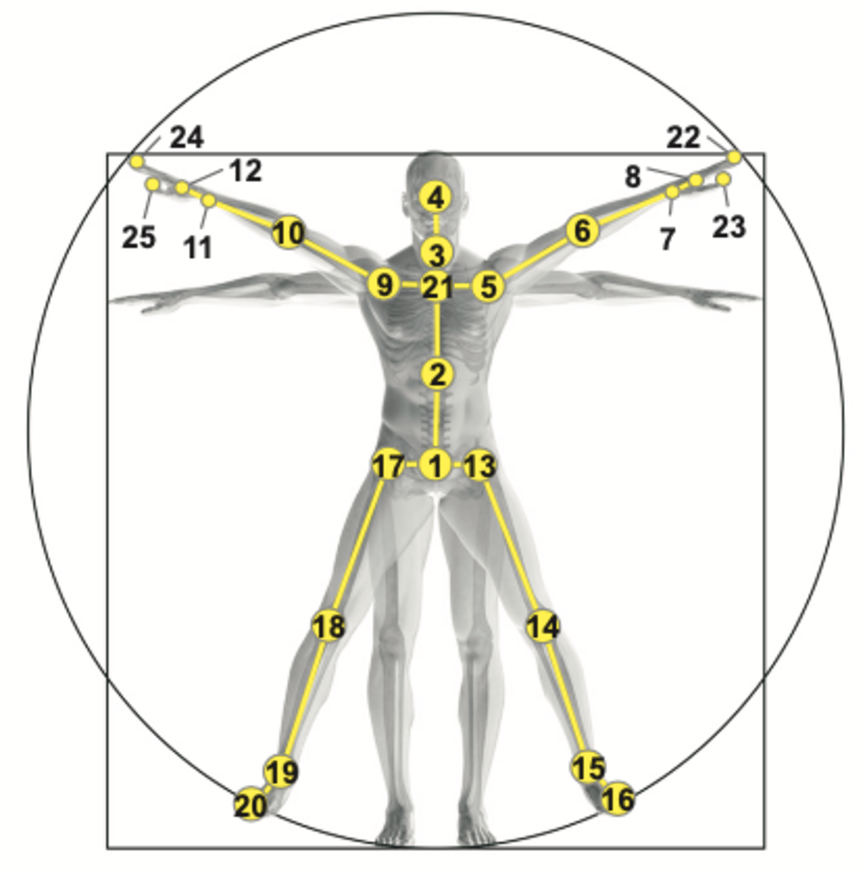
\includegraphics[width=0.7\textwidth]{images/joint_config.pdf}
            \caption{Joint configurations for NTU RGB-D dataset\footnotemark}
      \end{figure}      
      \end{columns}
      \footnotetext{A. Shahroudy, J. Liu, T.-T. Ng, and G. Wang, “NTU RGB+D: A Large Scale Dataset for 3D Human Activity Analysis,” in Proc. IEEE Conf. Computer Vision and Pattern Recognition (CVPR), 2016, pp. 1010–1019.}
\end{frame}

\begin{frame}{Action Recognition Analysis}
      \framesubtitle{}%
      
      \begin{itemize}
      \item Networks: CTR-GCN, MS-G3D, EfficientGCN, ViewAdaptive NN
      \item Joint, Bone and Joint Motions
      \item \textbf{Metrics}: Cross-Subject \& Training Time
      \end{itemize}
      \vfill
      \begin{table}[ht!]
      \centering
      {\footnotesize
      \begin{tabular}{ |c|c|c|c| } 
              \hline
              Drink Water & Eat Meal & Brush Teeth & Drop \\ 
              \hline
              Pick Up & Throw & Sit Down & Stand Up \\ 
              \hline
              Clapping & Hand Waving & Kick Something & Hopping \\ 
              \hline
              Jump Up & Play with Phone & Point to Something & Rub Hands \\
              \hline
              Nod Head/Bow & Shake Head & Wipe Face & Cross Hands \\
              \hline
      \end{tabular}
      }
      \caption{Subset of action classes from the NTU RGB-D dataset}
      \end{table}
\end{frame}

\begin{frame}{Action Recognition Analysis Results}
      \framesubtitle{}%
      
      \begin{columns}
      \column{.6\textwidth}
      \begin{table}[h!]
      \centering
      {\footnotesize
      \begin{tabular}{ |C{0.32\textwidth}|C{0.25\textwidth}|C{0.2\textwidth}| } 
              \hline
              \rowcolor{gray!25}
              Network & Cross Subject & Cross View \\ 
              \hline
              CTR-GCN (Joint) & 92.63\% & 96.37\% \\ 
              \hline
              CTR-GCN (Bone) & 92.78\% & 96.02\% \\ 
              \hline
              CTR-GCN (Motion) & 92.51\% & 96.40\% \\ 
              \hline
              MS-G3D (Joint) & 91.27\% & 96.85\% \\ 
              \hline
              MS-G3D (Bone) & 90.90\% & 95.44\% \\ 
              \hline
              EfficientGCN-B4 (SG Layer) & 94.05\% & 97.47\% \\ 
              \hline
              EfficientGCN-B4 (EpSep Layer) & 94.43\% & 97.56\% \\ 
              \hline
              VA-NN (CNN) & 92.97\% & 92.20\% \\
              \hline
      \end{tabular}
      }
      \caption{Action recognition networks accuracy}
      \end{table}
      
      \column{.4\textwidth}
      \begin{table}[h!]
      \centering
      {\footnotesize
      \begin{tabular}{ |c|c| }
              \hline
              \rowcolor{gray!25}
              Network & Training Time \\
              \hline
              CTR-GCN & 4 hrs\\
              \hline
              MS-G3D & 8 hrs\\
              \hline
              EfficientGCN-B4 & 5 hrs\\
              \hline
              VA-NN (CNN) & 0.5 hrs\\
              \hline
      \end{tabular}
      }
      \caption{Networks training time}     
      \end{table}
      \end{columns}
\end{frame}

\begin{frame}{Action Recognition Analysis Results}
      \framesubtitle{}%
      
      %\vspace{-0.25cm}
      \begin{table}[h!]
      \centering
      {\footnotesize
      \begin{tabular}{ | C{0.14\textwidth} | c | c | C{0.18\textwidth} | c | c | }
            \hline
            \rowcolor{gray!25}
            Action & CTR-GCN & MS-G3D & Action & CTR-GCN & MS-G3D \\
            \hline
            Drink Water & 82.48\% & 83.94\% & Kick Something & 97.83\% & 94.93\% \\
            \hline
            Eat Meal & 78.91\% & 73.82\% & Hopping & 98.91\% & 95.27\%  \\
            \hline
            Brush Teeth & 90.84\% & 91.21\% & Jump Up & 98.91\% & 98.55\% \\
            \hline
            Drop & 90.18\% & 91.64\% & Play with Phone & 86.91\% & 90.91\% \\
            \hline
            Pick Up & 98.91\% & 94.55\% & Point to Something & 92.39\% & 92.03\% \\
            \hline
            Throw & 96.36\% & 90.91\% & Rub Hands & 90.58\% & 89.49\% \\
            \hline
            Sit Down & 98.90\% & 97.80\% & Nod Head/Bow & 96.01\% & 95.65\% \\
            \hline
            Stand Up & 98.17\% & 98.90\% & Shake Head & 96.00\% & 95.64\% \\
            \hline
            Clapping & 82.42\% & 72.89\% & Wipe Face & 92.39\% & 94.20\% \\
            \hline
            Hand Waving & 94.16\% & 94.89\% & Cross Hands & 93.84\% & 94.57\% \\
            \hline
      \end{tabular}
      }
      \caption{Cross-Subject accuracy results per class for CTR-GCN and MS-G3D models}
      \end{table}
\end{frame}

\section{Comparative Analysis: Class-Incremental Learning}

\begin{frame}{Incremental Learning}
      \framesubtitle{}%
      
      \begin{block}{Class-Incremental Learning Problem}
            \small An algorithm that learns a given sequence of tasks, T:
            \begin{equation}
            \centering
            T = [ (C^1, D^1), (C^2, D^2), \ldots ,(C^n, D^n) ]
            \end{equation}
      \end{block}
      \vfill
      \begin{columns}
      \column{.55\textwidth}
      
      \begin{block}{Tasks}
            \small
            \begin{itemize}
            \item Set of actions to be learnt:
            \begin{equation}
            \centering
            D^t = \{ (x_1, y_1), \ldots, (x_{m^t}, y_{m^t}) \}
            \end{equation}
            \item Action set is distinct per task
            \begin{equation}
            \centering
            C^i \cap C^j = \oslash, \; if \; i \ne j
            \end{equation}
            \end{itemize}
      \end{block}
      
      \column{.45\textwidth}
      
      \begin{block}{Exemplars}
            \small
            \begin{itemize}
            \item Memory of training data from previous tasks
            \item Augments to training data if $t > 0$
            \item Memory scenarios: fixed or growing
            \item Selection methods: random, herding, distance, entropy
            \end{itemize}
      \end{block}
      
      \end{columns}
\end{frame}

\begin{frame}{Incremental Learning Metrics}
      \framesubtitle{}%
      
      \vspace{-0.35cm}
      \begin{columns}
      \column{.5\textwidth}
      \begin{block}{Task-Aware Accuracy}
            \small Calculated with the knowledge of the action classes learnt within each task.
      \end{block}
      \begin{block}{Task-Agnostic Accuracy}
            \small Calculated with the overall set of the action classes learnt.
      \end{block}
      
      \column{.5\textwidth}
      \begin{block}{Forgetting Percentage}
            \small Estimated percentage of data forgotten
            \begin{equation}
            \centering
            F_{i, t} = max(A[i, 0:t-1]) - A[i, t], \; i\leq t
            \end{equation}
      \end{block}
      
      \end{columns}
      \vfill
      \begin{figure}[ht!]
            \centering
            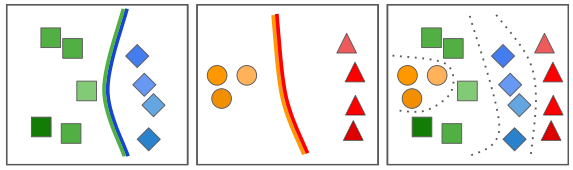
\includegraphics[width=0.45\textwidth]{images/IL_tasks}
            \caption{Incremental learning process of 4 classes split into 2 tasks\footnotemark}
      \end{figure} 
      \footnotetext{M. Masana et al., “Class-Incremental Learning: Survey and Performance Evaluation,” CoRR, vol. abs/2010.15277, October 2020.}
\end{frame}

\begin{frame}{Incremental Learning Analysis}
      \framesubtitle{}%
      
      \begin{columns}
      \column{0.3\textwidth}
      \vspace{-0.75cm}
      \begin{itemize}
            \item IL Algorithms: LwF, iCaRL, LUCIR, BiC
            \item Memory Size:\\ 400 (Fixed) \& 20 per class (Growing)
            \item Selection Method: Random \& Herding
            \item \textbf{Metrics}: Task-Aware \& Task-Agnostic Accuracy
      \end{itemize}
      
      \column{0.65\textwidth}
      \begin{table}[ht!]
      \centering
      {\footnotesize
      \begin{tabular}{ | c | C{0.24\textwidth} | c | C{0.28\textwidth} | }
            \hline
            \rowcolor{gray!25}
            Task \# & Action & Task \# & Action \\
            \hline
            Task 1 & Wipe Face & Task 6 & Throw \\
                        & Eat Meal & & Point to Something \\ 
            \hline
            Task 2 & Cross Hands & Task 7 & Hand Waving \\ 
                        & Clapping & & Stand Up \\
            \hline
            Task 3 & Kick Something & Task 8 & Nod Head/Bow \\
                        & Shake Head & & Hopping \\
            \hline
            Task 4 & Sit Down & Task 9 & Drop \\
                        & Play with Phone & & Drink Water \\
            \hline
            Task 5 & Pick Up & Task 10 & Rub Hands \\
                        & Brush Teeth & & Jump Up \\
            \hline
      \end{tabular}
      }
      \caption{Task sequence for class-IL comparative analysis}
      \end{table}
      \end{columns}
\end{frame}

\begin{frame}{Incremental Learning Analysis}
      \framesubtitle{LwF, iCaRL, LUCIR Model Architecture}%
      
      \vspace{0.5cm}
      {\footnotesize
      \centering
      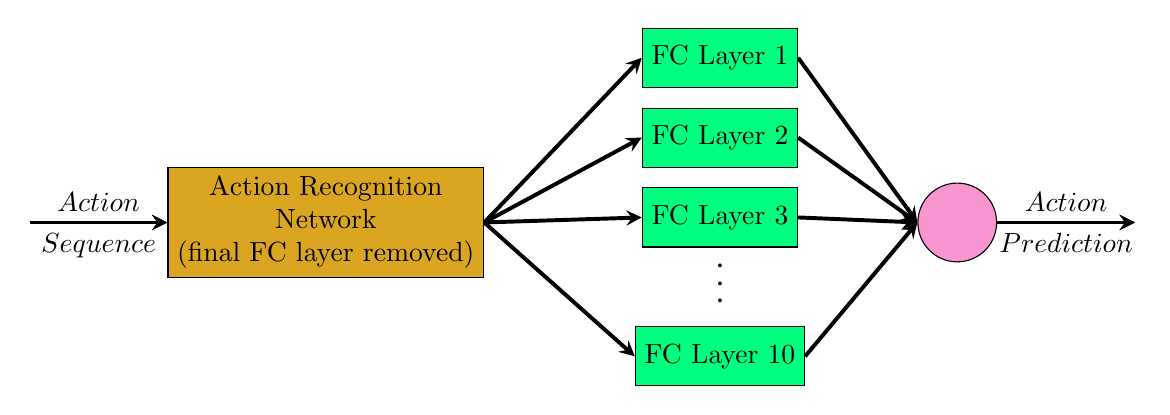
\begin{tikzpicture}
              \node[draw, align=center, fill=Goldenrod, minimum width=1cm, minimum height=1.2cm]  (net) at (0,0) {Action Recognition\\ Network\\ (final FC layer removed)};
              
              \node[draw, align=center, fill=SpringGreen, minimum width=1.5cm, minimum height=0.75cm, above right= 1cm and 2cm of net]  (head1) {FC Layer 1};
              \node[draw, align=center, fill=SpringGreen, minimum width=1.5cm, minimum height=0.75cm, below=0.25cm of head1]  (head2) {FC Layer 2};
              \node[draw, align=center, fill=SpringGreen, minimum width=1.5cm, minimum height=0.75cm, below=0.25cm of head2]  (head3) {FC Layer 3};
              \node[draw, align=center, fill=SpringGreen, minimum width=1.5cm, minimum height=0.75cm, below=1cm of head3]  (headt) {FC Layer 10};
              
              \node[draw, circle, minimum size=1cm, fill=Rhodamine!50, right= 5.5cm of net] (sum) {};
                            
              \path (head3) -- (headt) node [black, font=\Large, midway, sloped] {$\dots$};              
              \draw[stealth-,  line width=0.05cm] (net.west) -- ++ (-1.75,0) node[midway,above]{$Action$};
              \draw[stealth-,  line width=0.05cm] (net.west) -- ++ (-1.75,0) node[midway,below]{$Sequence$};
              
              \draw[-stealth,  line width=0.05cm] (net.east) -- (head1.west);
              \draw[-stealth,  line width=0.05cm] (net.east) -- (head2.west) node[midway,above]{};
              \draw[-stealth,  line width=0.05cm] (net.east) -- (head3.west) node[midway,above]{};
              \draw[-stealth,  line width=0.05cm] (net.east) -- (headt.west) node[midway,above]{};
                            
              \draw[-stealth,  line width=0.05cm] (head1.east) -- (sum.west) node[midway,above]{};
              \draw[-stealth,  line width=0.05cm] (head2.east) -- (sum.west) node[midway,above]{};
              \draw[-stealth,  line width=0.05cm] (head3.east) -- (sum.west) node[midway,above]{};
              \draw[-stealth,  line width=0.05cm] (headt.east) -- (sum.west) node[midway,above]{};
              
              \draw[-stealth,  line width=0.05cm] (sum.east) -- ++ (1.75,0) node[midway,above]{$Action$};
              \draw[-stealth,  line width=0.05cm] (sum.east) -- ++ (1.75,0) node[midway,below]{$Prediction$};
      \end{tikzpicture}
      }
\end{frame}

\begin{frame}{Incremental Learning Analysis}
      \framesubtitle{BiC Model Architecture}%
      
      \vspace{0.5cm}
      {\footnotesize
      \centering
      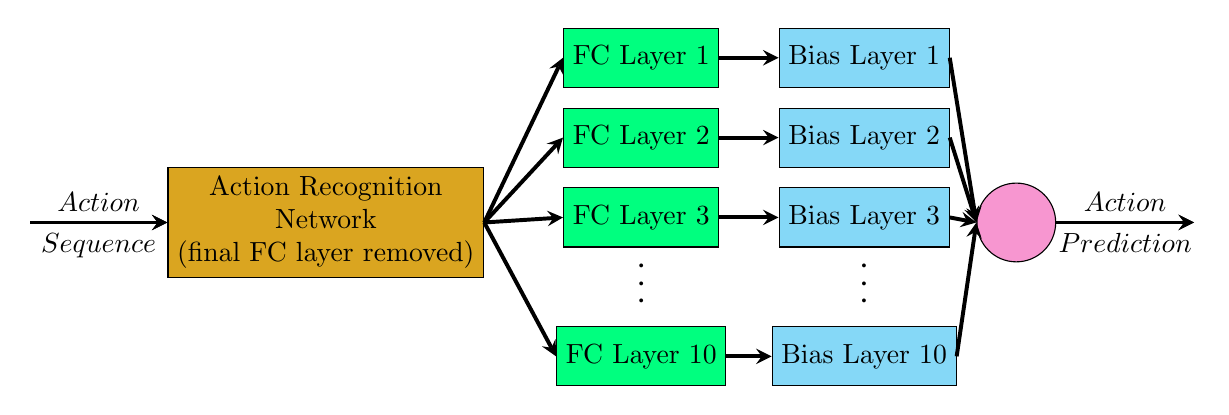
\begin{tikzpicture}
              \node[draw, align=center, fill=Goldenrod, minimum width=1cm, minimum height=1.2cm]  (net) at (0,0) {Action Recognition\\ Network\\ (final FC layer removed)};
              
              \node[draw, align=center, fill=SpringGreen, minimum width=1.5cm, minimum height=0.75cm, above right= 1cm and 1cm of net]  (head1) {FC Layer 1};
              \node[draw, align=center, fill=SpringGreen, minimum width=1.5cm, minimum height=0.75cm, below=0.25cm of head1]  (head2) {FC Layer 2};
              \node[draw, align=center, fill=SpringGreen, minimum width=1.5cm, minimum height=0.75cm, below=0.25cm of head2]  (head3) {FC Layer 3};
              \node[draw, align=center, fill=SpringGreen, minimum width=1.5cm, minimum height=0.75cm, below=1cm of head3]  (headt) {FC Layer 10};
              
              \node[draw, align=center, fill=ProcessBlue!50, minimum width=1.5cm, minimum height=0.75cm, right= 0.75cm of head1]  (bl1) {Bias Layer 1};
              \node[draw, align=center, fill=ProcessBlue!50, minimum width=1.5cm, minimum height=0.75cm, below=0.25cm of bl1]  (bl2) {Bias Layer 2};
              \node[draw, align=center, fill=ProcessBlue!50, minimum width=1.5cm, minimum height=0.75cm, below=0.25cm of bl2]  (bl3) {Bias Layer 3};
              \node[draw, align=center, fill=ProcessBlue!50, minimum width=1.5cm, minimum height=0.75cm, below=1cm of bl3]  (blt) {Bias Layer 10};
              
              \node[draw, circle, minimum size=1cm, fill=Rhodamine!50, right= 6.25cm of net] (sum) {};
                            
              \path (head3) -- (headt) node [black, font=\Large, midway, sloped] {$\dots$};
              \path (bl3) -- (blt) node [black, font=\Large, midway, sloped] {$\dots$};
              
              \draw[stealth-,  line width=0.05cm] (net.west) -- ++ (-1.75,0) node[midway,above]{$Action$};
              \draw[stealth-,  line width=0.05cm] (net.west) -- ++ (-1.75,0) node[midway,below]{$Sequence$};
              
              \draw[-stealth,  line width=0.05cm] (net.east) -- (head1.west);
              \draw[-stealth,  line width=0.05cm] (net.east) -- (head2.west) node[midway,above]{};
              \draw[-stealth,  line width=0.05cm] (net.east) -- (head3.west) node[midway,above]{};
              \draw[-stealth,  line width=0.05cm] (net.east) -- (headt.west) node[midway,above]{};
                            
              \draw[-stealth,  line width=0.05cm] (head1.east) -- (bl1.west) node[midway,above]{};
              \draw[-stealth,  line width=0.05cm] (head2.east) -- (bl2.west) node[midway,above]{};
              \draw[-stealth,  line width=0.05cm] (head3.east) -- (bl3.west) node[midway,above]{};
              \draw[-stealth,  line width=0.05cm] (headt.east) -- (blt.west) node[midway,above]{};
              
              \draw[-stealth,  line width=0.05cm] (bl1.east) -- (sum.west) node[midway,above]{};
              \draw[-stealth,  line width=0.05cm] (bl2.east) -- (sum.west) node[midway,above]{};
              \draw[-stealth,  line width=0.05cm] (bl3.east) -- (sum.west) node[midway,above]{};
              \draw[-stealth,  line width=0.05cm] (blt.east) -- (sum.west) node[midway,above]{};
              
              \draw[-stealth,  line width=0.05cm] (sum.east) -- ++ (1.75,0) node[midway,above]{$Action$};
              \draw[-stealth,  line width=0.05cm] (sum.east) -- ++ (1.75,0) node[midway,below]{$Prediction$};
      \end{tikzpicture}
      }
\end{frame}

\begin{frame}{Incremental Learning Analysis Results}
      \framesubtitle{}%
      
      %\vspace{-0.65cm}
      \begin{table}[ht!]
      \centering
      {\footnotesize
      \begin{tabular}{ | >{\columncolor{gray!25}}c | >{\columncolor{gray!25}}C{1.2cm} | C{1.37cm} | C{1.55cm} | C{1.3cm} | C{1.37cm} | C{1.55cm} | C{1.3cm} | }
            \hline
            \rowcolor{gray!25}
            & & \multicolumn{3}{c |}{CTR-GCN} & \multicolumn{3}{c |}{MS-G3D} \\
            \hline
            \rowcolor{gray!25}
            Algorithm & Memory Config & Total Time (hrs) & Time per Task (min) & Time Incr per Task & Total Time (hrs) & Time per Task (min) & Time Incr per Task \\
            \hline
            iCaRL & Fixed & 6.3 & 18.9 \& 39.2 & - & 11.2 & 30.2 \& 68.7 & - \\
            \cline{2-8}
            & Growing & 5.6 & - & 2.8\% & 11.0 & - & 2.6\% \\
            \hline
            LWF & Fixed & 6.6 & 19.9 \& 41.8 & - & 11.3 & 30.6 \& 69.6 & - \\
            \cline{2-8}
            & Growing & 5.8 & - & 2.8\% & 10.1 & - & 2.9\% \\
            \hline
            BIC & Fixed & 7.0 & \cellcolor{blue!25}19.6 \& 44.1 & - & 11.5 & 30.2 \& 68.2 & - \\
            \cline{2-8}
            & Growing & 6.2 & - & \cellcolor{blue!25}3.3\% & 10.4 & - & 2.6\% \\
            \hline
            LUCIR & Fixed & 6.4 & 19.6 \& 39.6 & - & 11.4 & 33.0 \& 71.4 & - \\
            \cline{2-8}
            & Growing & 5.8 & - & 2.9\% & 10.1 & - & 2.9\% \\
            \hline
      \end{tabular}
      }
      \caption{Incremental learning model training time}
      \end{table}
\end{frame}

\begin{frame}{Incremental Learning Analysis Results}
      \framesubtitle{}%
      
      \begin{table}[ht!]
      \centering
      {\footnotesize
      \begin{tabular}{ | >{\columncolor{gray!25}}c | >{\columncolor{gray!25}}C{1.2cm} | C{1.55cm} | C{1.55cm} | C{1.55cm} | C{1.55cm} | }
            \hline
            \rowcolor{gray!25}
            & & \multicolumn{2}{c |}{Herding} & \multicolumn{2}{c |}{Random} \\
            \hline
            \rowcolor{gray!25}
            Algorithm & Memory Config & CTR-GCN & MS-G3D  & CTR-GCN & MS-G3D \\
            \hline
            iCaRL & Fixed & 94.9\% & 97.2\% & 95.3\% & 98.1\% \\
            \cline{2-6}
            & Growing & 91.1\% & 95.9\% & 91.2\% & 96.6\% \\
            \hline
            LWF & Fixed & 98.4\% & 97.8\% & 98.2\% & 97.5\% \\
            \cline{2-6}
            & Growing & 97.6\% & 96.1\% & 97.1\% & 96.1\% \\
            \hline
            LUCIR & Fixed & 95.5\% & 97.5\% & 97.3\% & 97.5\% \\
            \cline{2-6}
            & Growing & 96.3\% & 94.8\% & 95.5\% & 96.5\% \\
            \hline
            BiC & Fixed & \cellcolor{blue!25}98.2\% & 98.1\% & 97.9\% & 96.9\% \\
            \cline{2-6}
            & Growing & \cellcolor{blue!25}97.3\% & 96.9\% & 97.5\% & 96.6\% \\
            \hline
      \end{tabular}
      }
      \caption{Average task-aware accuracy }
      \end{table}
\end{frame}

\begin{frame}{Incremental Learning Analysis Results}
      \framesubtitle{}%
      
      \begin{table}[ht!]
      \centering
      {\footnotesize
      \begin{tabular}{ | >{\columncolor{gray!25}}c | >{\columncolor{gray!25}}C{1.2cm} | C{1.55cm} | C{1.55cm} | C{1.55cm} | C{1.55cm} | }
            \hline
            \rowcolor{gray!25}
            & & \multicolumn{2}{c |}{Herding} & \multicolumn{2}{c |}{Random} \\
            \hline
            \rowcolor{gray!25}
            Algorithm & Memory Config & CTR-GCN & MS-G3D  & CTR-GCN & MS-G3D \\
            \hline
            iCaRL & Fixed & 52.1\% & 72.5\% & 50.9\% & 72.1\% \\
            \cline{2-6}
            & Growing & 54.2\% & 67.8\% & 51.3\% & 66.9\% \\
            \hline
            LWF & Fixed & 73.8\% & 67.8\%  & 75.4\% & 67.5\% \\
            \cline{2-6}
            & Growing & 69.9\% & 61.5\% & 69.4\% & 63.5\% \\
            \hline
            LUCIR & Fixed & 66.2\% & 64.7\% & 68.4\% & 64.4\% \\
            \cline{2-6}
            & Growing & 65.5\% & 43.6\% & 62.4\% & 59.9\% \\
            \hline
            BiC & Fixed & \cellcolor{blue!25}79.1\% & 70.1\% & 74.8\% & 67.1\% \\
            \cline{2-6}
            & Growing & \cellcolor{blue!25}74.2\% & 61.1\% & 72.8\% & 61.6\% \\
            \hline
      \end{tabular}
      }
      \caption{Average task-agnostic accuracy}
      \end{table}
\end{frame}

\begin{frame}{Incremental Learning Analysis}
      \framesubtitle{How would the model perform if we grouped similar actions?}%
      
      \vspace{0.25cm}
      \begin{columns}
      \column{0.5\textwidth}
      \begin{itemize}
            \item Task-Aware Accuracy: 
            \begin{itemize}
                  \item \small Fixed: 98.2\% $\Longrightarrow$ 94.6\%
                  \item \small Growing: 97.3\% $\Longrightarrow$ 93.4\%
            \end{itemize}
      \end{itemize}
      \column{0.5\textwidth}
      \begin{itemize}
            \item Task-Agnostic Accuracy: 
            \begin{itemize}
                  \item \small Fixed: 79.1\% $\Longrightarrow$ 77.6\%
                  \item \small Growing: 74.2\% $\Longrightarrow$ 72.7\%
            \end{itemize}
      \end{itemize}
      \end{columns}
      \vspace{0.5cm}
      \begin{table}[ht!]
      \centering
      {\footnotesize
      \begin{tabular}{ | c | c | c | c | c | c | }
            \hline
            \rowcolor{gray!25}
            Task \# & Action & Task \# & Action & Task \# & Action \\
            \hline
            Task 1 & Brush Teeth & Task 4 & Sit Down & Task 7 & Kick Something \\
            & Wipe Face & & Stand Up & & Hopping \\
            \cline{1-4}
            Task 2 & Drink Water & Task 5 & Clapping & & Jump Up \\
            \cline{5-6}
            & Eat Meal & & Rub Hands & Task 8 & Play with Phone \\
            \cline{1-2}
            \cline{5-6}
            Task 3 & Drop & & Cross Hands & Task 9 & Nod Head/Bow \\
            \cline{3-4}
            & Pick Up & Task 6 & Hand Waving & & Shake Head \\
            & Throw & & Point to Something & & \\
            \hline
      \end{tabular}
      }
      \caption{Task sequence with variable task size and sorting similar actions}
      \end{table}
\end{frame}

\begin{frame}{Incremental Learning Analysis}
      \framesubtitle{Model Robustness}%
      
      \vspace{0.25cm}
      \begin{columns}
      \column{0.5\textwidth}
      \begin{itemize}
            \item Task-Aware Accuracy: 
            \begin{itemize}
                  \item \small Fixed: 94.6\% $\Longrightarrow$ 94.1\% \& 96.7\%
                  \item \small Growing: 93.4\% $\Longrightarrow$ 95.1\% \& 95.6\%
            \end{itemize}
      \end{itemize}
      \column{0.5\textwidth}
      \begin{itemize}
            \item Task-Agnostic Accuracy: 
            \begin{itemize}
                  \item \small Fixed: 77.6\% $\Longrightarrow$ 76.3\% \& 78.5\%
                  \item \small Growing: 72.7\% $\Longrightarrow$ 74.5\% \& 70.6\%
            \end{itemize}
      \end{itemize}
      \end{columns}
      \vspace{0.6cm}
      {\footnotesize
      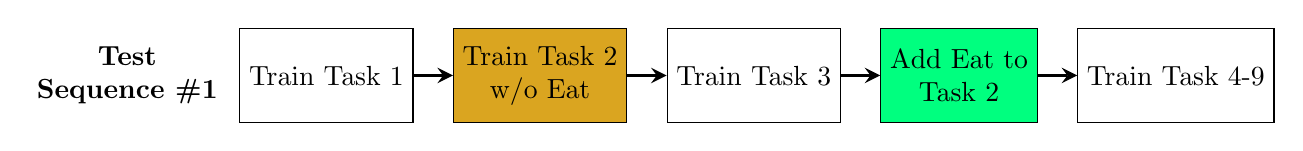
\begin{tikzpicture}
            \node[align=center, fill=white, minimum width=1cm, minimum height=1.2cm]  (t0) at (0,0) {\textbf{Test}\\ \textbf{Sequence \#1}};
            \node[draw, align=center, fill=white, minimum width=1cm, minimum height=1.2cm, right=0.15cm of t0] (t1) {Train Task 1};
            \node[draw, align=center, fill=Goldenrod, minimum width=1cm, minimum height=1.2cm, right=0.5cm of t1]  (t2) {Train Task 2\\ w/o Eat};
            \node[draw, align=center, fill=white, minimum width=1cm, minimum height=1.2cm, right=0.5cm of t2]  (t3) {Train Task 3};
            \node[draw, align=center, fill=SpringGreen, minimum width=1cm, minimum height=1.2cm, right=0.5cm of t3]  (t4) {Add Eat to\\ Task 2};
            \node[draw, align=center, fill=white, minimum width=1cm, minimum height=1.2cm, right=0.5cm of t4]  (t5) {Train Task 4-9};
            
            \draw[-stealth,  line width=0.05cm] (t1.east) -- (t2.west);
            \draw[-stealth,  line width=0.05cm] (t2.east) -- (t3.west);
            \draw[-stealth,  line width=0.05cm] (t3.east) -- (t4.west);
            \draw[-stealth,  line width=0.05cm] (t4.east) -- (t5.west);
      \end{tikzpicture}
      }
      \vspace{0.75cm}

      {\footnotesize
      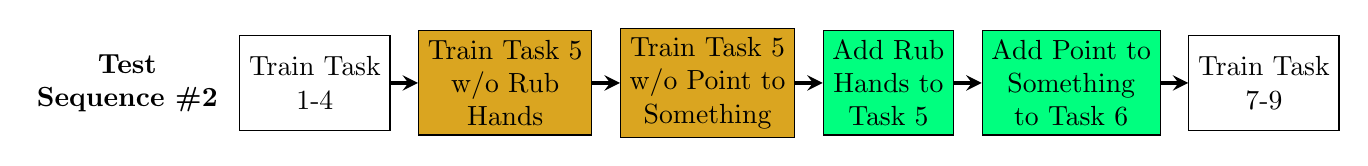
\begin{tikzpicture}
            \node[align=center, fill=white, minimum width=1cm, minimum height=1.2cm]  (t0) at (0,0) {\textbf{Test}\\ \textbf{Sequence \#2}};
            \node[draw, align=center, fill=white, minimum width=1cm, minimum height=1.2cm, right=0.15cm of t0] (t1) {Train Task\\ 1-4};
            \node[draw, align=center, fill=Goldenrod, minimum width=1cm, minimum height=1.2cm, right=0.35cm of t1]  (t2) {Train Task 5\\ w/o Rub\\ Hands};
            \node[draw, align=center, fill=Goldenrod, minimum width=1cm, minimum height=1.2cm, right=0.35cm of t2]  (t3) {Train Task 5\\ w/o Point to\\ Something};
            \node[draw, align=center, fill=SpringGreen, minimum width=1cm, minimum height=1.2cm, right=0.35cm of t3]  (t4) {Add Rub\\ Hands to\\ Task 5};
            \node[draw, align=center, fill=SpringGreen, minimum width=1cm, minimum height=1.2cm, right=0.35cm of t4]  (t5) {Add Point to\\ Something\\ to Task 6};
            \node[draw, align=center, fill=white, minimum width=1cm, minimum height=1.2cm, right=0.35cm of t5]  (t6) {Train Task\\ 7-9};
            
            \draw[-stealth,  line width=0.05cm] (t1.east) -- (t2.west);
            \draw[-stealth,  line width=0.05cm] (t2.east) -- (t3.west);
            \draw[-stealth,  line width=0.05cm] (t3.east) -- (t4.west);
            \draw[-stealth,  line width=0.05cm] (t4.east) -- (t5.west);
            \draw[-stealth,  line width=0.05cm] (t5.east) -- (t6.west);
      \end{tikzpicture}
      }
\end{frame}

\begin{frame}{Incremental Learning Analysis}
      \framesubtitle{Memory Size}%
      
      \begin{table}[ht!]
      \centering
      {\footnotesize
      \begin{tabular}{ | C{0.75cm} | C{0.75cm} | C{0.75cm} | C{0.75cm} | C{0.75cm} | C{0.75cm} | C{0.75cm} | C{0.75cm} | C{0.75cm} | C{0.75cm} | C{0.75cm} | }
            \hline
            \multicolumn{6}{| c |}{\cellcolor{gray!25}Growing} & \multicolumn{5}{c |}{\cellcolor{gray!25}Fixed} \\
            \hline
            2 & 5 & 10 & 20 & 50 & 100 & 40 & 100 & 200 & 400 & 1000 \\
            \hline
            78.3\% & 94.3\% & 97.2\% & \cellcolor{blue!25}97.3\% & 98.5\% & 98.7\% & 94.5\% & 96.7\% & 97.6\% & 98.2\% & 98.5\% \\
            \hline
      \end{tabular}
      }
      \caption{Average task-aware accuracy for varying memory size}
      \end{table}
      \vfill
      \begin{table}[ht!]
      \centering
      {\footnotesize
      \begin{tabular}{ | C{0.75cm} | C{0.75cm} | C{0.75cm} | C{0.75cm} | C{0.75cm} | C{0.75cm} | C{0.75cm} | C{0.75cm} | C{0.75cm} | C{0.75cm} | C{0.75cm} | }
            \hline
            \multicolumn{6}{| c |}{\cellcolor{gray!25}Growing} & \multicolumn{5}{c |}{\cellcolor{gray!25}Fixed} \\
            \hline
            2 & 5 & 10 & 20 & 50 & 100 & 40 & 100 & 200 & 400 & 1000 \\
            \hline
            11.3\% & 45.7\% & 63.8\% & \cellcolor{blue!25}74.2\% & 79.8\% & 84.1\% & 35.8\% & 65.2\% & 70.3\% & 79.1\% & 80.0\% \\
            \hline
      \end{tabular}
      }
      \caption{Average task-agnostic accuracy for varying memory size}
      \end{table}     
\end{frame}

\section{Assistive Robot Integration}

\begin{frame}{QTRobot Platform}
      \framesubtitle{}%
      
      \begin{columns}
      \column{0.5\textwidth}
      \begin{itemize}
            \item Teaching assistant for educators working with children
            \item Equipped with a RealSense 3D camera
            \item Skeletal tracking using Nuitrack SDK (19 joints tracked vs 25 joints in NTU)
      \end{itemize}

      \column{0.5\textwidth}
      \begin{figure}[ht!]
            \centering
            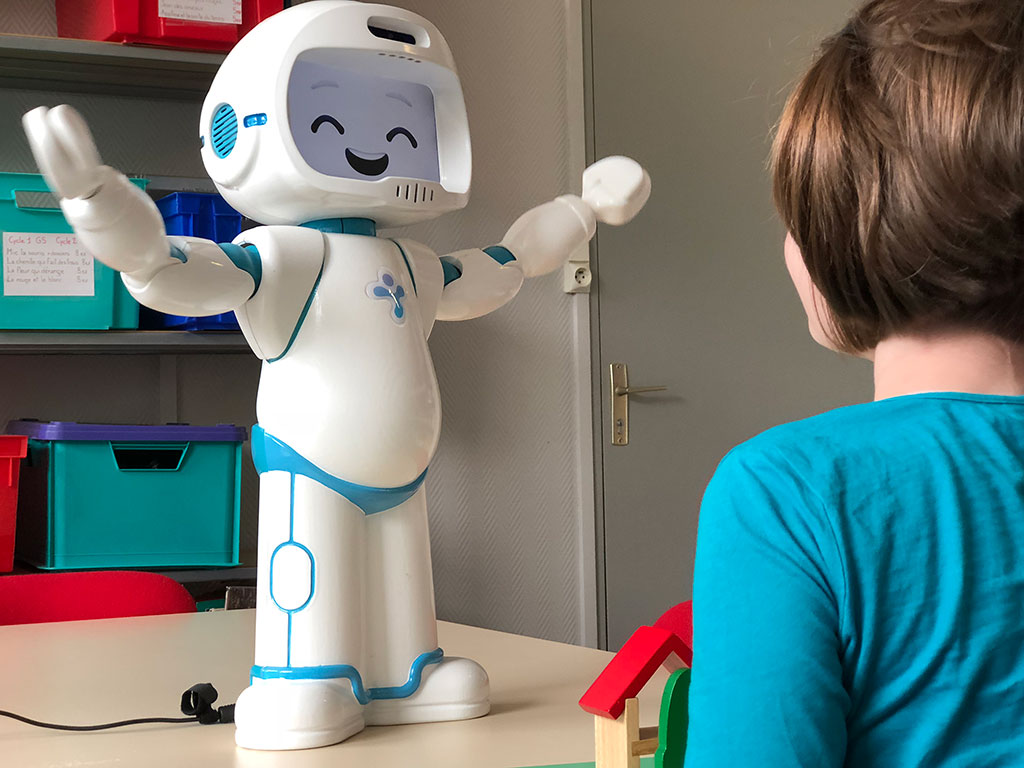
\includegraphics[width=0.8\textwidth]{images/qtrobot_with_child.jpeg}
            \caption{QTRobot interacting with a child\footnotemark}
      \end{figure}
      \end{columns}
      \footnotetext{Image taken from: https://robots.ieee.org/robots/qtrobot/} 
\end{frame}

\begin{frame}{Model Integration}
      \framesubtitle{}%
      
      \vspace{-0.3cm}
      \begin{columns}
      \column{0.55\textwidth}
       \begin{itemize}
            \item Task-Aware Accuracy: \small 97.3\% $\Longrightarrow$ 97.4\%
            \item Task-Agnostic Accuracy: \small 74.2\% $\Longrightarrow$ 71.9\%
      \end{itemize}
      \vspace{-0.25cm}
      \begin{figure}[h!]
      \centering
      \begin{tikzpicture}
              \node (a) {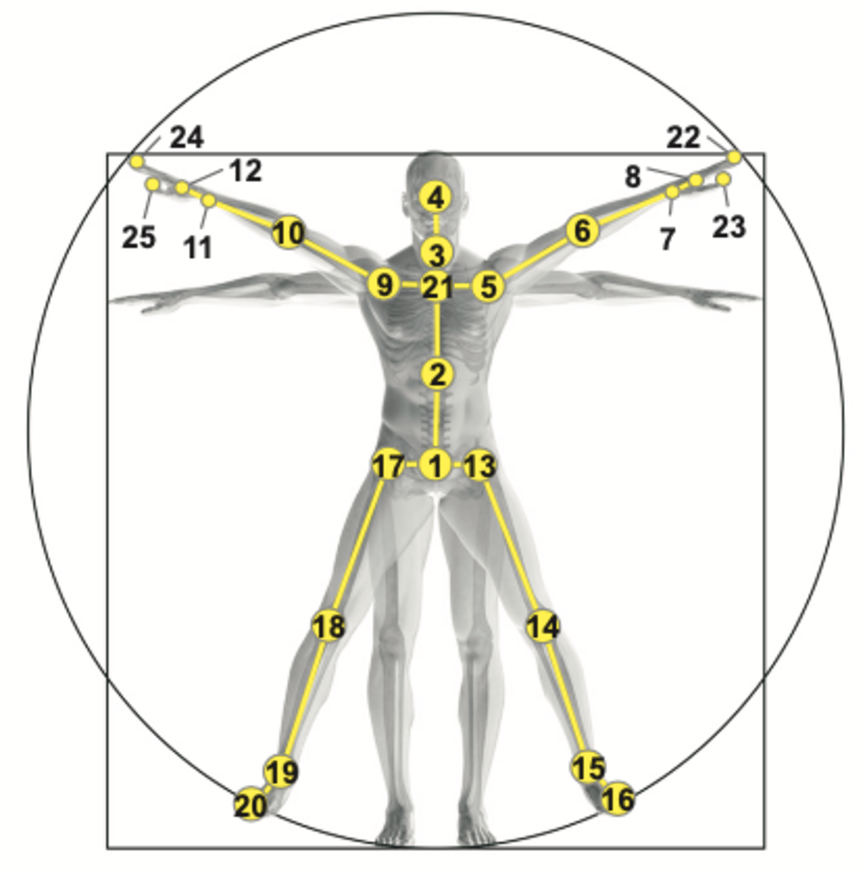
\includegraphics[trim=10 10 5 5,clip, width=0.475\textwidth]{images/joint_config.pdf}};
              
              \draw[red] (-1.1,1.29) circle (0.1cm and 0.1cm); %24
              \draw[red] (1.07,1.29) circle (0.1cm and 0.1cm); %22
              \draw[red] (-1.31,0.85) circle (0.1cm and 0.1cm); %25
              \draw[red] (1.28,0.89) circle (0.1cm and 0.1cm); %23
              \draw[red] (-0.82,-1.65) circle (0.1cm and 0.1cm); %20
              \draw[red] (0.79,-1.62) circle (0.1cm and 0.1cm); %16
      \end{tikzpicture}
      \caption{Joint configurations for NTU RGB-D dataset\footnotemark[6]}
      \end{figure} 
      
      \column{0.5\textwidth}
      \begin{figure}[ht!]
            \centering
            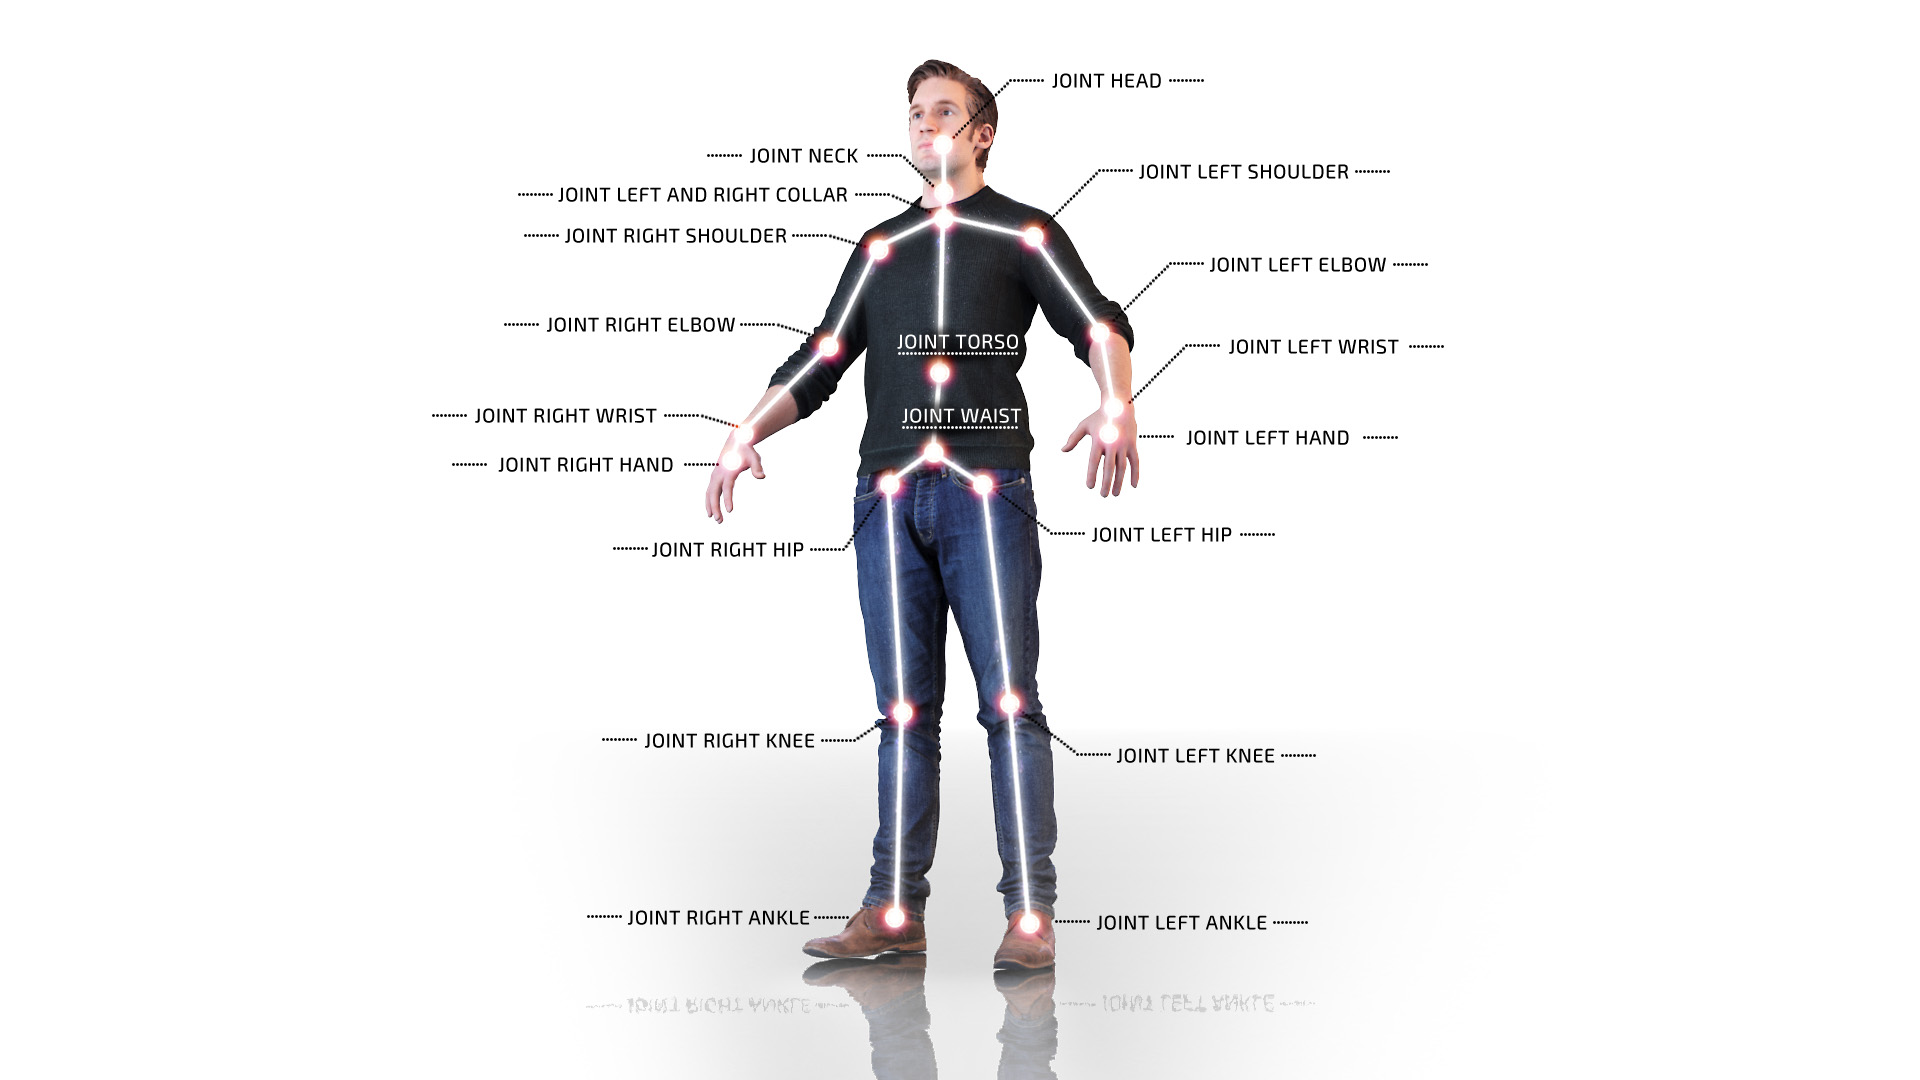
\includegraphics[trim=425 100 425 60,clip, width=0.8\textwidth]{images/nt_joints_config.jpeg}
            \caption{Joint configuration in the Nuitrack SDK\footnotemark[7]}
      \end{figure}
      \end{columns}
      \footnotetext[6]{A. Shahroudy, J. Liu, T.-T. Ng, and G. Wang, “NTU RGB+D: A Large Scale Dataset for 3D Human Activity Analysis,” in Proc. IEEE Conf. Computer Vision and Pattern Recognition (CVPR), 2016, pp. 1010–1019.}
      \footnotetext[7]{Image taken from: https://github.com/3DiVi/nuitrack-sdk/tree/master/doc}
\end{frame}

\begin{frame}{CAL Server}
      \framesubtitle{}%
      
      \begin{columns}
      \column{0.15\textwidth}

      \column{0.85\textwidth}
      \vspace{-1.25cm}
      \begin{figure}[ht!]
            \centering
            %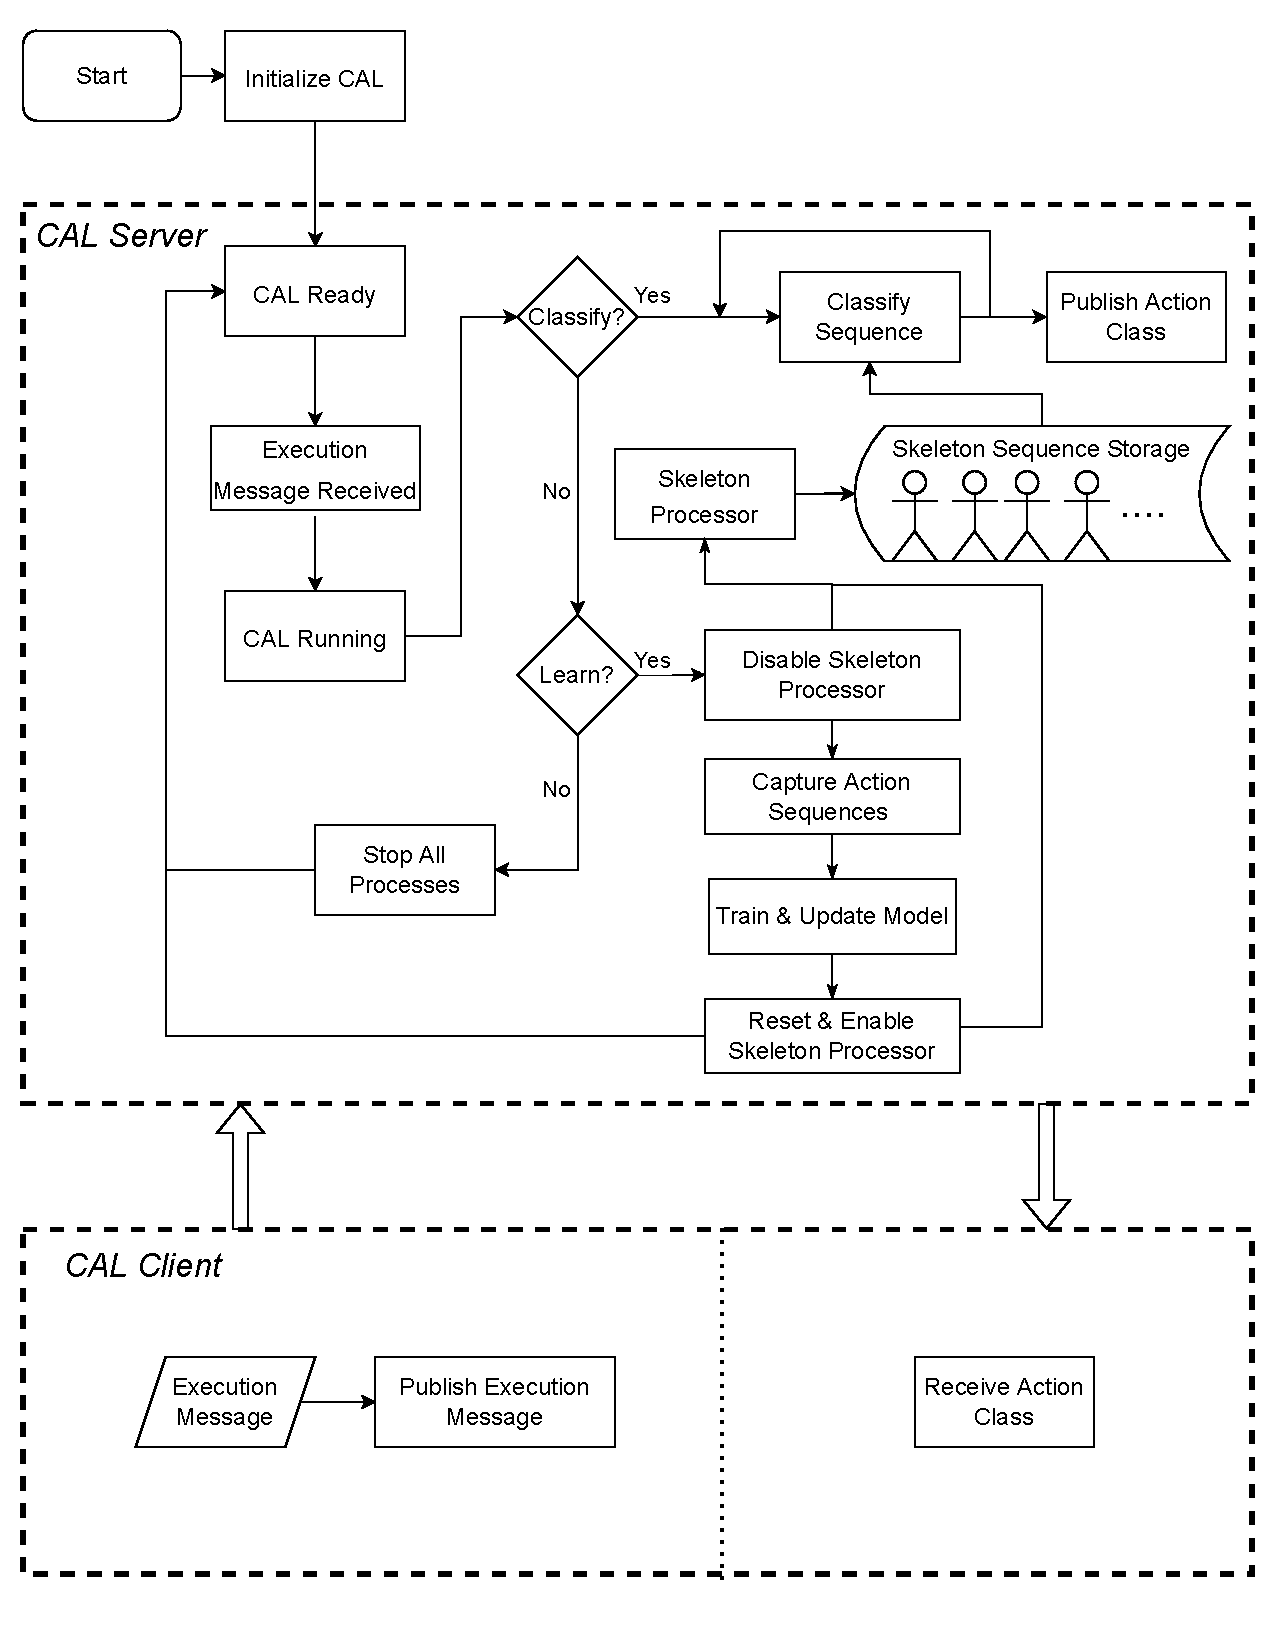
\includegraphics[trim=10 262 10 10,clip, width=0.7\textwidth]{images/CAL_workflow.pdf}
            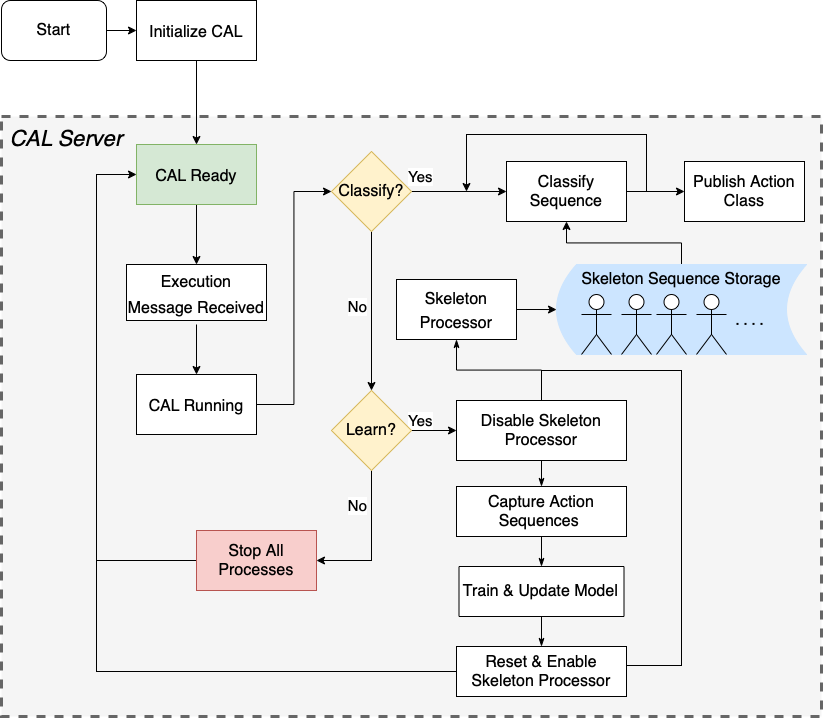
\includegraphics[width=0.7\textwidth]{images/CAL_workflow.png}
            \caption{Workflow of the Continual Action Learning Server}
      \end{figure}
      \end{columns}      
\end{frame}

\begin{frame}{Demo}
      \framesubtitle{Action Recognition}%
      
      %\movie[width=3cm,height=2cm,poster]{}{mymovie.mpg}
\end{frame}

\begin{frame}{Demo}
      \framesubtitle{Action Learning}%
      
      %\movie[width=3cm,height=2cm,poster]{}{mymovie.mpg}
\end{frame}

\begin{frame}
      \vspace{1.25cm}
      \centering
      \Huge
      \emph{Thank You!}\\
      \vspace{0.25cm}
      \large
      Questions?
\end{frame}



\end{document}
